%%%%%%%%%%%%%%%%%%%%%%%%%%%%%%%%%%%%%%%%%%%%%%%%%%%%%%%%%%%%%%%%%%%%%%%%%%%%%%%
%                                                                             %
% 06 - API Pública                                                            %
%                                                                             %
%%%%%%%%%%%%%%%%%%%%%%%%%%%%%%%%%%%%%%%%%%%%%%%%%%%%%%%%%%%%%%%%%%%%%%%%%%%%%%%

\chapter{\textcolor{azulescom}{API Pública}}

\section{Objetivo}
SkyPrice provee una API pública para aquellos usuarios que deseen integrar el
servicio de estimación de precio en sus propios proyectos. La API pública
se ofrece como un servicio gratuito y no requiere de registro previo para su uso.

\section{Acceso a la API}
Para acceder a la API pública de SkyPrice, simplemente se debe utilizar la URL:

\begin{center}
\texttt{http://api.skyprice.xyz}
\end{center}

Al acceder a la URL, el servicio responde con un mensaje inicial indicando detalles
generales de SkyPrice pero además se incluyen dos enlaces a la documentación de la API,
uno en formato Swagger UI y otro en formato ReDoc.

\section{Documentación}
SkyPrice provee de documentación en formato OpenAPI 3.0 para su API pública. La
documentación se encuentra disponible en dos formatos: Swagger UI y ReDoc. Para
acceder a la documentación, simplemente se debe utilizar los siguientes enlaces:

\begin{center}
\texttt{http://api.skyprice.xyz/openapi} \\
\texttt{http://api.skyprice.xyz/redoc}
\end{center}

En la figura \ref{fig:swagger} se muestra la interfaz de Swagger UI y en la figura
\ref{fig:redoc} se muestra la interfaz de ReDoc.

\begin{figure}[H]
\centering
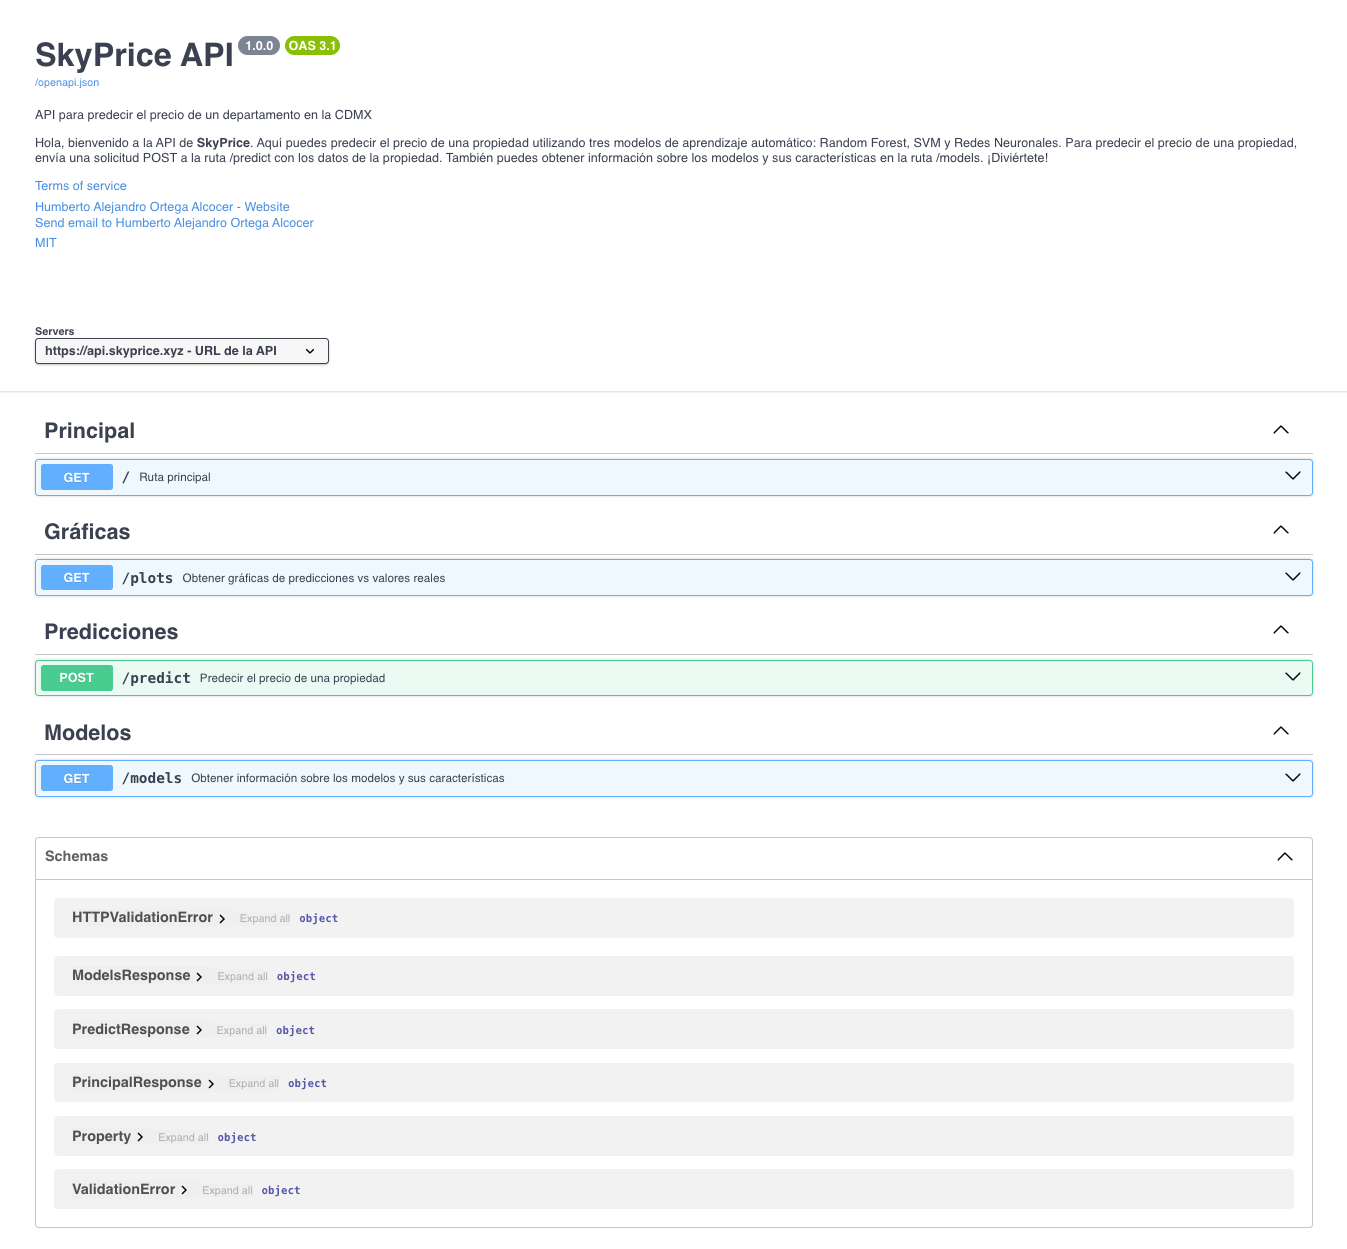
\includegraphics[width=0.9\textwidth]{imagenes/06-api-publica/swagger.png}
\caption{Interfaz de Swagger UI}
\label{fig:swagger}
\end{figure}

\begin{figure}[H]
\centering
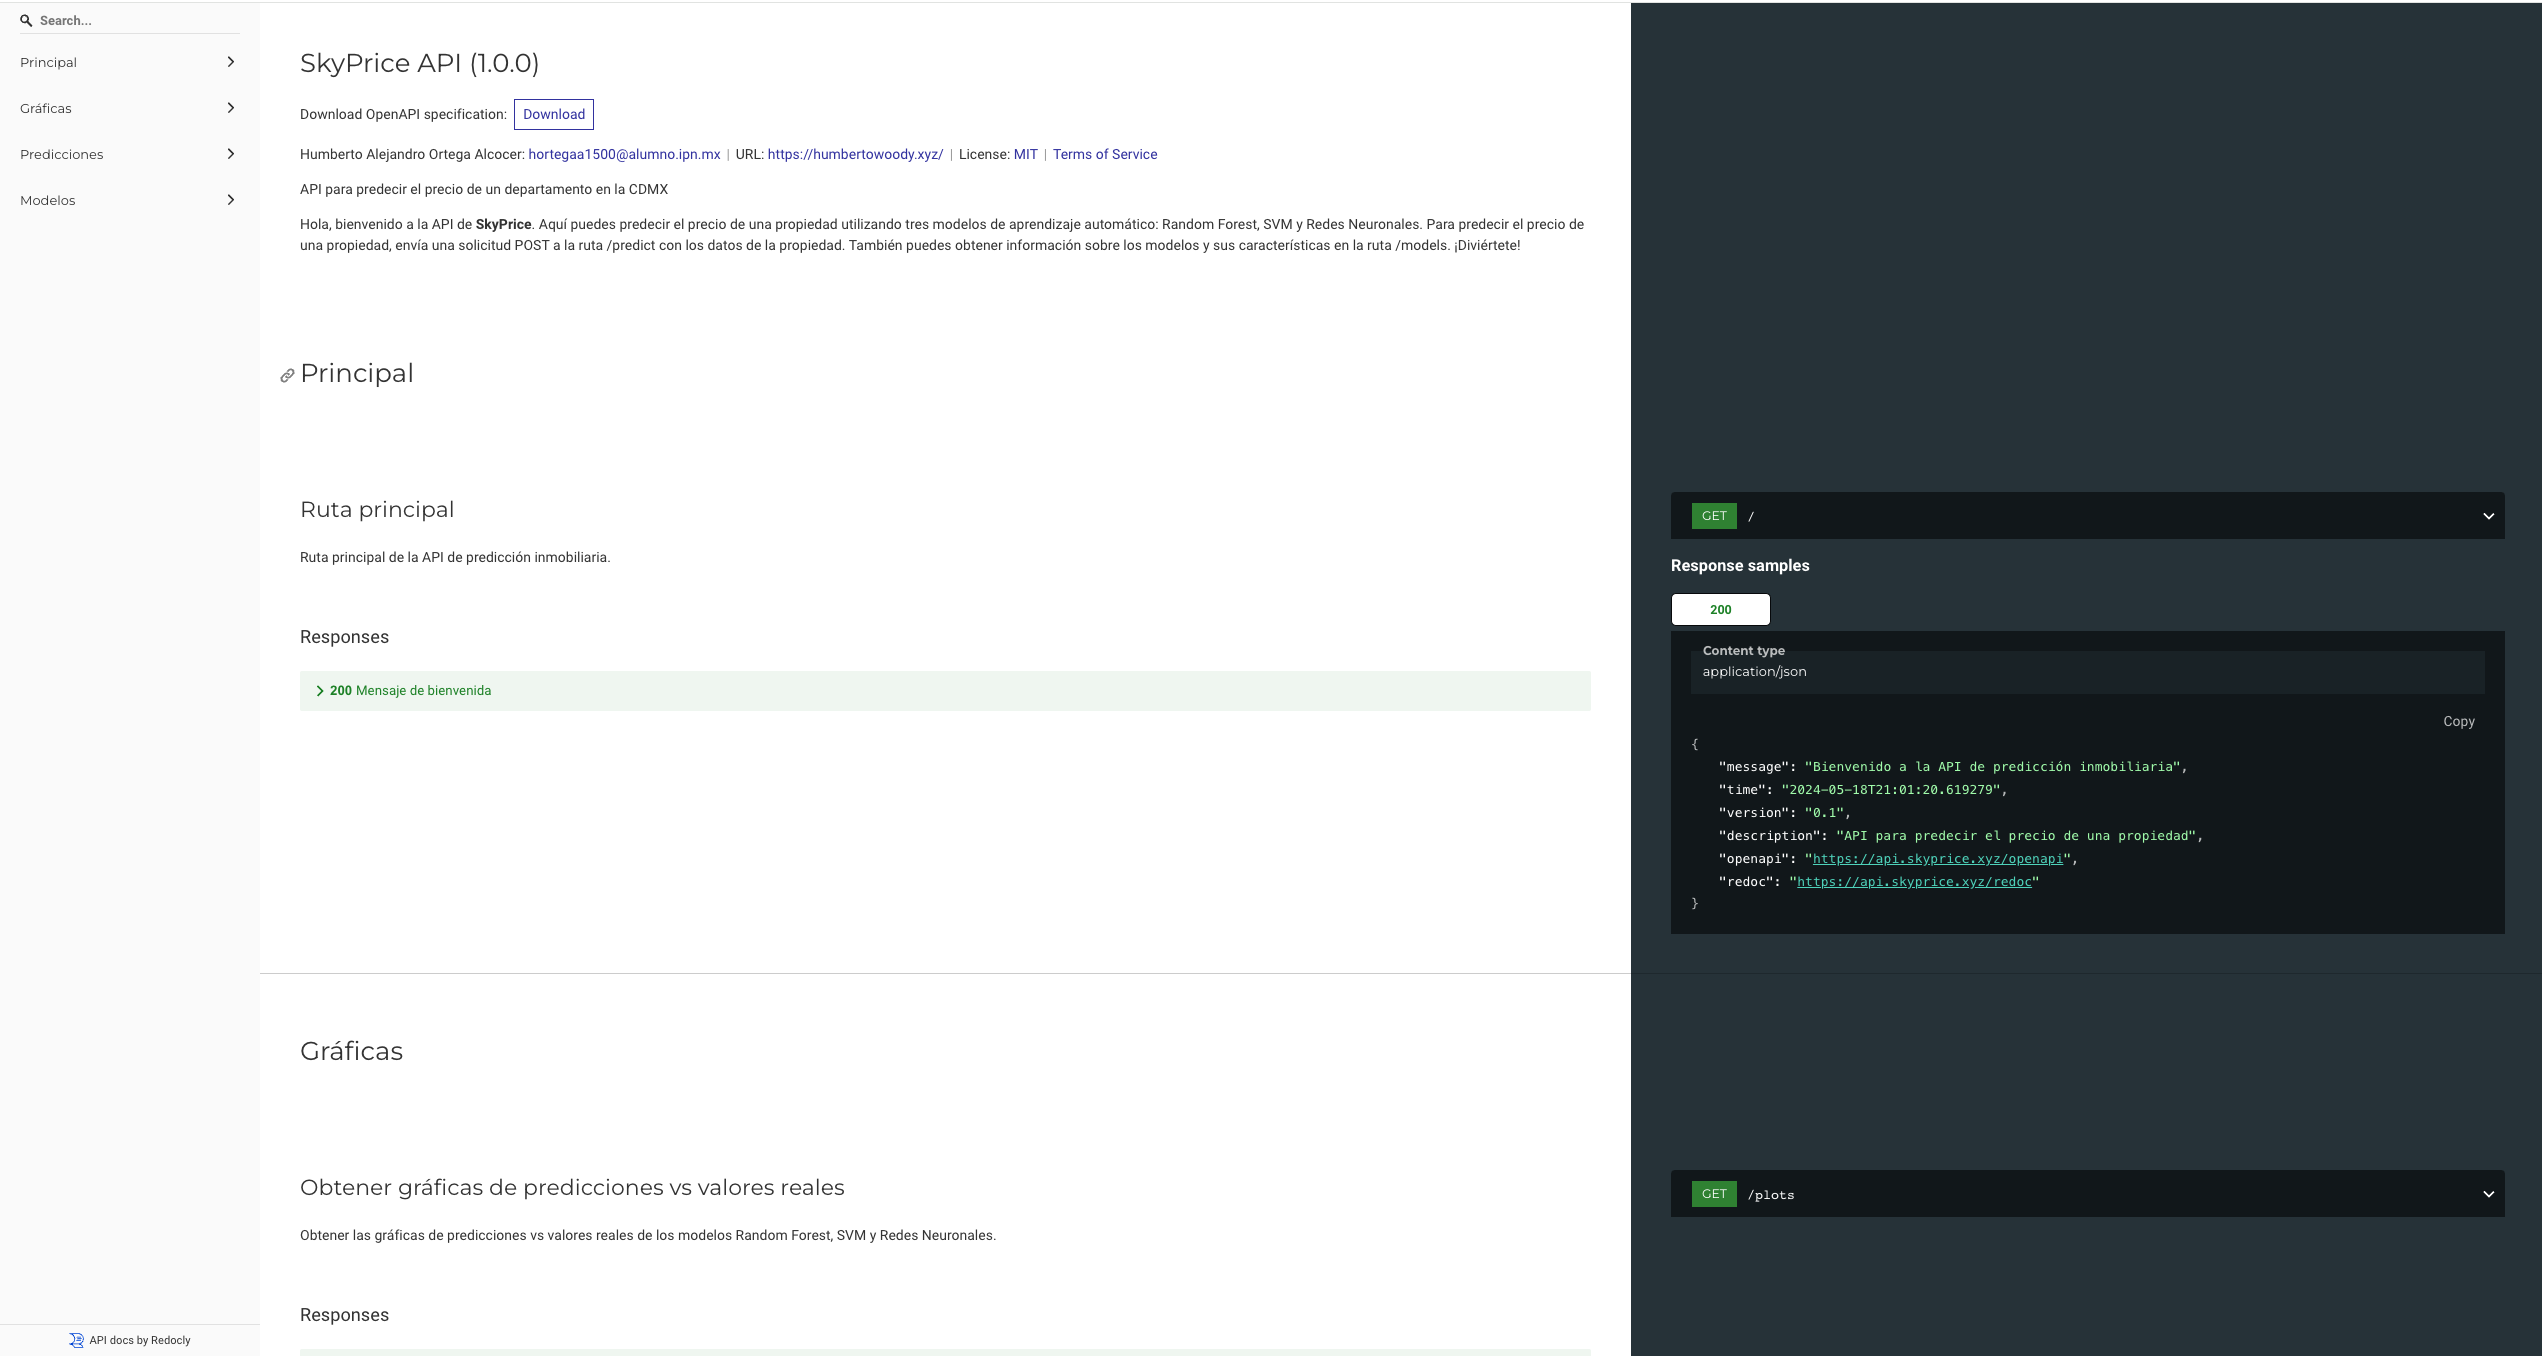
\includegraphics[width=0.9\textwidth]{imagenes/06-api-publica/redoc.png}
\caption{Interfaz de ReDoc}
\label{fig:redoc}
\end{figure}

\section{Estructura de la API}
La API cuenta con cuatro endpoints principales:

\begin{itemize}
\item \texttt{/} - Endpoint raíz de la API, provee detalles generales de SkyPrice
como el nombre del servicio, versión, hora actual del servidor, enlaces a la
documentación en formato swagger y redoc.
\item \texttt{/predict} - Endpoint para realizar una predicción de precio de un
departamento en base a sus características.
\item \texttt{/models} - Endpoint para obtener información de los modelos de
aprendizaje automático utilizados por SkyPrice.
\item \texttt{/plots} - Endpoint para obtener una gráfica de evaluación de los
modelos comparando el precio real con el precio de la predicción.
\end{itemize}

\section{Ejemplos de uso}
A continuación se presentan ejemplos de uso de la API pública de SkyPrice.

\begin{itemize}
\item \textbf{Predicción de precio de un departamento:} Se puede utilizar para
estimar el precio de uno o varios departamentos en la Ciudad de México.
\item \textbf{Información de los modelos:} Se puede utilizar para mostrar
de forma dinámica en alguna interfaz de usuario la información de los modelos o
para tomar decisiones sobre cuál modelo utilizar para las predicciones.
\item \textbf{Gráfica de evaluación de los modelos:} Se puede utilizar para
mostrar de forma dinámica en alguna interfaz de usuario la gráfica de evaluación
de los modelos.
\end{itemize}

\section{Errores}
La API pública de SkyPrice utiliza códigos de estado HTTP para indicar el resultado
de una petición. En caso de que ocurra un error, la API responderá con un código de
estado HTTP 4xx o 5xx y un mensaje de error en formato JSON. A continuación se
presentan los códigos de estado y mensajes de error posibles:

\begin{itemize}
\item \textbf{400 Bad Request:} La petición no pudo ser procesada debido a un error
en los datos enviados por el cliente.
\item \textbf{404 Not Found:} El recurso solicitado no fue encontrado en el servidor.
\item \textbf{500 Internal Server Error:} Ocurrió un error interno en el servidor.
\end{itemize}

\section{Límites de uso}
La API pública de SkyPrice no tiene límites de uso establecidos. Sin embargo, se
recomienda no realizar más de 1000 peticiones por minuto para evitar problemas de
rendimiento en el servidor.

\section{Seguridad}
La API pública de SkyPrice no requiere de autenticación para su uso. Sin embargo,
se recomienda utilizar HTTPS para proteger la comunicación entre el cliente y el
servidor.

\section{Política de uso}
La API pública de SkyPrice es un servicio gratuito y no requiere de registro previo
para su uso. Sin embargo, se espera que los usuarios hagan un uso responsable de la
API y respeten los límites de uso establecidos.

\section{Contacto}
Para cualquier duda o comentario sobre la API pública de SkyPrice, se pone a
disposición el siguiente correo electrónico:

\begin{center}
api@skyprice.xyz
\end{center}


